\documentclass{article}

\usepackage{amsmath}
\usepackage{graphicx}
\graphicspath{}

\usepackage[citestyle=authoryear, style=authoryear]{biblatex}
\addbibresource{paper2.bib}

\title{An agent-based model of military mechanization}

\author{Tom Wallace}

\begin{document}

\maketitle

\begin{centering}
	Word count: XXXX
\end{centering}
\section{Introduction}

This paper presents an agent-based model of military mechanization. First, it
provides a theoretical discussion of military mechanization, states the research
hypothesis, and explains why agent-based modeling is an appropriate research strategy.
Then, it details an original agent-based model; presents results; and discusses
their implications for the academic debate on military mechanization.

In summary, the orthodox view of military mechanization is that it is a
reflexive process: states choose their mechanization posture largely based on
that neighbors, enemies, and recent military experiences (e.g. defeat in
counter-insurgency). This paper argues
that this view---based on traditional longitudinal data analysis---is ripe for
agentization. It implicitly argues for autonomous agents (states) that have
cognition regarding mechanization that takes into account other agents (e.g.
enemies), spatiality (e.g. neighbors), and learning from experience. This paper
builds such a model and validates it against the empirical record, using the
National Mechanization Index of \cite{sechser2010army}. It finds that the 
orthodox view of mechanization does not stand up to agentization. A positive feedback loop exists causes states to
mechanize much faster and to a greater degree than occurs in the real-world.
This implies the existence of some countervailing factor (possibly a negative
feedback loop) that mitigates the extent of mechanization. Candidates for what
this could be mostly center on ``internal'' factors---e.g., culture, economy,
and so on---as opposed to the ``external'', security environment-centric
orthodox view.

\section{Background}

\subsection{Military mechanization}

States differ in the composition of their military ground forces.\footnote{States may have multiple organizations that
conduct ground combat operations: e.g., the United States operates both an Army
and a Marine Corps as independent services. Henceforth, this paper uses the
terms ``army'' and ``ground forces'' interchangeably.} One notable axis of comparison 
is \textit{mechanization}: the degree to which an army consists of infantry 
vs. combat vehicles. Treating mechanization as a continuous variable, 
one extreme is an army consisting exclusively of dismounted, small 
arms-wielding infantry units; the other extreme is an army consisting 
solely of tank units, armored personnel carriers, artillery, and the like.
Clearly, no modern state embodies either extreme, but the 1970s-era Vietcong are
a good example of a low-mechanization army and the 1980s-era Israeli army of
high mechanization.

The consequences of mechanization are large. There is
academic consensus that defense policy---including but not limited to
mechanization---conditions battlefield effectiveness. 
\cite{lyall2009rage} finds that highly mechanized militaries are less effective
at counterinsurgency, while \cite{biddle2004military} argues that
mechanization-enabled mobility aids conventional warfighting. It thus
pays to have an army that is designed to win the
kinds of
conflicts that a state is likely to face. Lacking a crystal ball, however,
leaders cannot always forecast conflict, and armies are large, complex
organizations that typically are held to change only infrequently and slowly (\cite{murray1998military},
\cite{locher2004victory}, \cite{zegart2000flawed}). A state suddenly faced with
a war for which its mechanization posture is ill-suited can either concede or
pay a cost in blood and treasure; what it cannot do is
quickly overcome the constraints imposed by past mechanization decisions. 
A quote from then-Secretary of Defense Donald Rumsfeld---made in 2004, when the U.S. military
was confronted in Iraq with the consequences of past choices regarding
mechanization---emphasizes the point:
``you go to war with the army you have'' (\cite{schmitt_2004}). 

The causes of military mechanization are disputed. \textit{Realists} believe 
that mechanization choices are driven by security environment. States
choose mechanization policies that they believe will allow them to prevail against potential adversaries, or to send a
signal of deterrence, or to learn from the perceived mistakes of the last war
(\cite{mearsheimer1983conventional};
\cite{huth1988extended}; \cite{murray2011military}). The other school of thought is more
diverse and so harder to name, but may be termed 
\textit{institutionalists}. They believe that factors other than 
strategic calculation determine military mechanization. Domestic political
institutions---e.g., democracy vs. autocracy, politically stable vs.
coup-prone, the state of civil-military relations, and so on---may influence 
force structure (\cite{reiter2002democracies}; \cite{quinlivan1999coup};
\cite{talmadge2015dictator}; \cite{brooks2008shaping}). Economic factor
endowments may play a role: e.g., capital-rich states may mechanize more
than labor-rich states (\cite{gartzke2001democracy}). Lastly,
ideology (\cite{van1984cult}) and culture (e.g., \cite{pollack2004arabs}) are
hard-to-measure but perhaps influential. Consider Ireland: between the 1920s and
1940s, it expended a large portion of its defense budget on building
a small number of tanks. They were wholly insufficient to repel a British 
invasion (their ostensible purpose), and
Ireland would have been better-served to pursue a low-mechanization guerrilla
defense strategy, but tanks were seen as a prestigious signifier of a ``real''
professional military, an important factor for the young Irish state
(\cite{farrell1998professionalization};
\cite{farrell2001transnational}).

\cite{sechser2010army} is the landmark study on military mechanization. They
assemble a longitudinal dataset at the country-year level of the mechanization
of all states between 1979 and 2001, and conduct regression analysis to identify
the effect of covariates on mechanization. They conclude that ``choices about
mechanization are strongly associated with a state's security environment.''
The more mechanized a state's geographic neighbors and enemies, the higher the state's 
own mechanization; also, states
learn from defeat in insurgency by subsequently decreasing their mechanization.

\subsection{The case for agent-based modeling}

The findings of \cite{sechser2010army} are ripe for agentization. The
conclusions drawn implicitly claim
that states are autonomous agents; that they have
cognition regarding how to perceive the outside world
and how to react to it; that spatiality and
neighborhood matter; that inter-agent relationships matter; and that
agents learn from experience. Agent-based modeling is uniquely well-suited to
represent such phenomena (\cite{gilbert2005simulation};
\cite{miller2009complex}).

Importantly, the findings of \cite{sechser2010army} imply a positive feedback
loop. State A has high
mechanization, causing enemy State B to raise their mechanization, causing State
A to raise their mechanization... and so on. Such feedback loops are a hallmark
of complex systems and again are well-suited for representation by agent-based
modeling. This specific one---states changing their military in response to
other states change in military in response to... and so on---feedback loop---is often called
the ``security dilemma'' and was a main research interest of Thomas Schelling, one of the pioneers
of agent-based modeling (\cite{schelling1960strategy};
\cite{schelling2006micromotives}).

\subsection{Research question and strategy}

I hypothesize that the arguments of \cite{sechser2010army} are incomplete and
that some omitted variable(s) act(s) as a ``brake'' on 
mechanization.\footnote{By ``omitted'', I mean that they conclude that the variable
is not very important for mechanization, not that they do not address the
variable at all.} An agent-based model is used to test this hypothesis. In broad
terms, agents (states) are defined to have the cognitive and learning behavior
implicitly claimed by \cite{sechser2010army}. The model is initialized with
real-world data from 1979 and allowed to run until 2001. The micro- and
macro-outcomes are then validated against real-world 2001 data. If
\cite{sechser2010army} are correct, the model's 2001 outcomes should match
real-world 2001 outcomes. If the model mechanization levels in 2001 are much
higher, then their claimed behavioral rules are incomplete and fail to include
some ``brake'' on mechanization, matching my hypothesis. Proving exactly what
that missing variable or set of variables is is outside the scope of this model
and paper, though it is discussed.

\section{Model}

This section of the paper describes the model. It does not use the ODD protocol
of \cite{grimm2006standard} but covers many of the same points.

\subsection{Agents}

There is one agent type: states. Agents exist at a fixed location and do not
move. The set of agents encompasses all diplomatically-recognized 
states in the world at a particular point in time, minus microstates (defined as
those with a population less than 750,000). Some other states were excluded; for
why, see the \textbf{Time}
section. Figure 1 depicts the set of agents.

\begin{figure}[h!]
	\centering
	\caption{Agents}
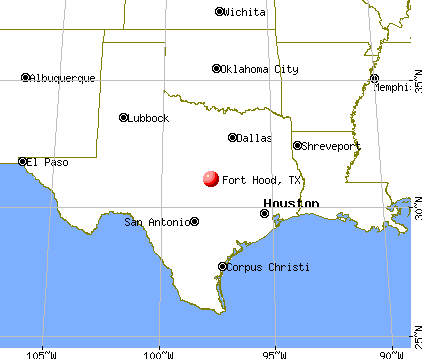
\includegraphics[scale=0.05]{map.png}
\end{figure}

Agents have attributes. \textit{Name} is self-explanatory.
\textit{Mechanization} is the agent's level of mechanization at a given
timestep. Mechanization is calculated as the number of armored vehicles per 100
soldiers, per \cite{sechser2010army}. \textit{Neighbors} is a list containing
the \textit{Names} of an agent's geographic neighbors at a given point in
time---more on this in the subsequent \textbf{Environment} section. \textit{NeighborsMech} is the
average mechanization level of an agent's \textit{Neighbors} at a given point in
time. \textit{Enemies} is a list containing the \textit{Names} of an agent's
enemies at a given point in time. An enemy is an agent with which the agent in
question has had a militarized interstate dispute in the preceding ten years,
per the Correlates of War (COW) Militarized Interstate Disputes Database (MIDB)
(\cite{cow_midb}). \textit{EnemiesMech} is the average mechanization score of
enemies. Agents also have attributes that affect their
perception of other agents and cognition for changing their own behavior. These
attributes are discussed in the \textbf{Cognition and Actions} section.


\subsection{Environment}

Agents exist in a spatial environment. Spatiality is represented by neighbor
relationships. Two states are defined as
being neighbors if they share a contiguous land border or a stretch of water
less than 400 miles. Data on neighbor relationships is taken from the Correlates
of War (COW) Direct Continuity dataset (\cite{cow_contiguity}).
Modeling spatiality as dyadic neighbor relationships, rather than a more
detailed raster or vector GIS implementation, is justified on the basis that the
academic literature on mechanization suggests that two states neighboring each
other is the important factor, not more detailed geographic information (e.g.,
topographical features along the border). As such, this paper's modeling choice
captures the phenomenon of interest while avoiding the overhead of a full-blown
GIS implementation coupled with ABM
(e.g., \cite{harper2002modeling}).

\subsection{Cognition}

Agents have global perception of other agents: they can ``see'' the
mechanization state of all other agents. This modeling choice is reflective of
the real world, in which states devote significant resources to stay informed of
the military posture of others. Agent cognition centers on 
updating their own mechanization in response to the external security
environment. This occurs in three ways. One, if an agent's
\textit{NeighborsMech} increases---i.e., the agent's neighbors become more
mechanized---the agent will increase its own mechanization by some proportional
amount controlled by the agent's unique \textit{NeighborMechSensitivity}
attribute, which is heterogenous across agents (more on this below).
Two, if an agent's
\textit{EnemiesMech} increases---i.e., the agent's enemies become more
mechanized---the agent will increase its own mechanization by some proportional
amount controlled by the agent's unique \textit{EnemyMechSensitivity} attribute,
again heterogenous across agents. Three,
agents occasionally suffer an ``anti-mechanization lesson'': defeat in a
counter-insurgency conflict. Such events are scripted to occur for agents and
years as per the historical record: e.g., the Soviet Union experienced such a
lesson in the 1980s in Afghanistan. An agent experiencing such an event will
decrease their own mechanization by some amount controlled by the agent's
unique \textit{LessonSensitivity} attribute, again heterogenous across agents.
Cognition for agent $i$ thus is:

\begin{multline}
\textrm{Mech}_i^{(t+1)} = \textrm{Mech}_i^{(t)} \\ 
+ (\textrm{NeighborMechSensitivity}_i \times \textrm{NeighborMech}_i^{(t)}) \\
+ (\textrm{EnemyMechSensitivity}_i \times \textrm{EnemyMech}_i^{(t)}) \\
	+ (\textrm{LessonSensitivity}_i \times I_{\textrm{Lesson}}(t, i))
\end{multline}

with $(t)$ denoting timestep, $i$ indexing agents, and $I_{\textrm{Lesson}}(t,
i)$ an indicator function of whether the agent experienced an anti-mechanization
lesson. Table 1 summarizes agent attributes.

\begin{table}[h]
	\centering
	\caption{Attributes, organized by theme}
	\begin{tabular}{|l l|}
		\hline
		\textbf{Identity} & \textit{Name} \\
		& \\
		\textbf{Mechanization} & \textit{Mechanization} \\
		& \\
		\textbf{Spatiality} & \textit{Neighbors} \\
		& \\
		\textbf{Inter-agent Relationships} & \textit{Enemies} \\
		& \\
		\textbf{Perception} & \textit{EnemiesMech} \\
		& \textit{NeighborsMech} \\
		& \textit{Lesson} \\
		& \\
		\textbf{Cognition} & \textit{EnemyMechSensitivity} \\
		& \textit{NeighborsMechSensitivity} \\
		& \textit{LessonSensitivity} \\
		\hline
	\end{tabular}
\end{table}

An important note is that these three factors---neighbors, enemies, and
defeat in counter-insurgency---correspond to the factors identified by 
\cite{sechser2010army} as most important for mechanization. Because the research
goal is essentially to see whether their findings stand up to agentization,
it is critical to make agent cognition work in about the way that their findings
predict. Inclusion of other factors not identified as important for
mechanization---e.g., alliances, economic factors,
culture, etc.---would be interesting but counter-productive to the research
question. They are discussed along with this model's findings. 

Data for \textit{NeighborsMechSensitivity}, \textit{EnemiesMechSensitivity}, and
\textit{LessonSensitivity} come from \cite{sechser2010army}. Specifically, they
estimate coefficients and standard errors for these three factors, thus defining
a statistical distribution for each. Upon instantiation, every agent makes a
random draw from each of the three distributions, the resulting values of are
taken for these three attributes. This modeling choice has two important
elements. One, it further enhances agent heterogeneity. Agents already differ in
their geographic neighbors, enemies, and experiences with anti-mechanization
lessons; now, they also differ in the cognition used to update mechanization
based on these factors. It also introduces a stochastic element to the
model, meaning that each run differs and so multiple runs must be conducted for
each specification.

\subsection{Time}

The model starts in 1979 and runs in 2-year time increments until 2001. This
timespan and periodicity reflects data availability: a longer time period and
more frequent updates would be ideal but is not practically achievable. Agent
attributes are initialized, and then then the model iterates through timesteps. 
In discussing what happens each timestep, it is useful to distinguish between
things that depend on agents' actions and those that do not.

Some changes are deterministically programmed into the model and do not depend on
agent behavior. Every timestep, neighbor relationships and enemy relationships
are updated in accordance with the historical record. The occurrence of
counter-insurgency defeats also is hardwired into the model and does not depend
on agent behavior within the model.

Other changes do depend on agent behavior. Agent activation order in a
particular timestep is random. Every timestep, every agent perceives the world
aorund them; recalculates \textit{NeighborsMech} and \textit{EnemiesMech};
updates their mechanization level according to \textit{NeighborMechSensitivity}
and \textit{EnemyMechSensitivity}; and updates their mechanization level
according to \textit{LessonSensitivity} if an anti-mechanization lesson occured.

An important caveat is that the set of agents represented in the model does not
change over time: i.e., agents are the same from 1979 onwards. In real life,
of course, the agent population was not static over this time period, with many
states ceasing to exist in 1991 and new ones forming. Modeling these changes is
beyond the scope of this model. How a collapsed state's military assets are divvied up
among successor states is complex and not tractable to simple representation
(e.g. averaging). For example, the Soviet Union deployed most of its modern
military equipment in the far west of the country in anticipation of a conflict
with NATO, and so when the USSR collapsed Ukraine inherited the lion's share, leaving
little for successor states like Kazakhstan or Azerbaijan (\cite{roy1993military}). Such inheritance has
a strong effect on the mechanization of of successor states. Designing
complex and state-specific ``rules of inheritance'' was too much for this
initial effort but is an area for further development.

\subsection{Output Data, Verification, and Validation}

The main model output of interest is data on military mechanization. It is provided for
every agent and every time-step. These agent-level data also can be aggregated
into system-level measures of military mechanization. Per the research design,
the intent is to compare the model output to what actually occurred. If the
model produces military mechanization levels much higher than reality, it means
that Sechser and Saunder's findings do not stand up to agentization and there is
some missing ``brake'' on military mechanization. Note that this research
strategy has validation (comparison of model output to empirical data) at its
core and so no separate validation is needed. Verification that the model is
doing what it is intended was accomplished through manual inspection.

\section{Results}

\subsection{System-Level}

\subsection{Agent-Level}

\section{Discussion}

Learning ala \cite{bennett2006modelling}

\printbibliography[heading=bibnumbered]

\end{document}
